\section{Screening a Laplace insertion}
\label{sec:screening}

Reflection nullity is an unconditional plane identity. We now strengthen it
to an identity conditional on all exterior spins. The distinction matters:
conditioning on one spin and its edge decoration does not specify the other
spin. The proof has three steps. We move separated, arbitrarily rare block
patterns by positive normal transfers; we include the finitely many colors
that can transmit information through their buffers; and we join the blocks
by short open wires, protected by surrounding circuits.

All lengths in this section are physical lengths. Every layout, including
its smallest gaps, is fixed before the mesh tends to zero. We use the neutral
nodal discretization of \cref{sec:spectral}. In particular,
\begin{equation}
 X_\delta=K_\delta(\Delta\phi),\qquad
 \phi\in C_c^\infty(B),
 \label{eq:screen-insertion}
\end{equation}
has coefficients of exactly zero sum and is a function of increments in a
fixed arbitrarily small enlargement of $B$. The plane law is denoted by
$\P_\delta$. Its two spins and the decoration are denoted by $(s,d,W)$ as
in \cref{lem:finite-cuts}; $N$ is the dual complement of $W$.

\begin{proposition}[Exterior orthogonality]
\label{prop:screened-orthogonality}
Let $Q$ be a square and let $B$ be a concentric disk whose radius is less
than one thousandth of the side length of $Q$. For
$\phi\in C_c^\infty(B)$, let $\mathscr E_\delta(Q)$ be the sigma-field
generated by the full pair of spins outside $Q$, the $W$ states on
mutually dual edge pairs whose incident corner-grid plaquette is disjoint
from $Q$ (and hence the corresponding $N$ states), and all height
increments computable there. Then
\begin{equation}
 \left\|\E_{\P_\delta}
       [X_\delta\mid\mathscr E_\delta(Q)]\right\|_1
       \longrightarrow0.
 \label{eq:plane-exterior-orthogonality}
\end{equation}
The same assertion holds under any sequence of flat-domain laws having a
fixed larger square $Q^+$ compactly in their interiors, with
$\overline Q\subset Q^+$. It is uniform over those domains, including
the component laws supplied by an earlier exact flat cut. In the latter
case it is applied to the conditional law at that cut, before any later
data are revealed. Additive height constants do not affect the assertion.
\end{proposition}

\subsection{Uniform bounds under separated patterns}

A block pattern specifies all $s$ spins and all $W$ edges of a finite
regular block, including both endpoints of every specified edge. Blocks
will have pairwise disjoint filled isolating neighborhoods; a slightly
smaller compact core in each block is reserved for observing $d$ colors.
The blocks and their neighborhoods can have finitely many predetermined
indentations. Constants may depend on this geometry, but never on the
number of microscopic values in a pattern. Write $P_i$ for a specified
pattern in block $i$, and $p_i=\P_\delta(P_i)>0$.

\begin{lemma}[Neutral insertion moments under patterns]
\label{lem:screen-pattern-moments}
Suppose a smooth neutral insertion $Y_\delta=K_\delta(f)$ has a filled
pin-free neighborhood with positive clearance from finitely many pattern
neighborhoods. For every finite $p$,
\begin{equation}
 \E\bigl[|Y_\delta|^p\mid P_1\cap\cdots\cap P_m\bigr]
       \le C_p.
 \label{eq:screen-pattern-moment}
\end{equation}
The estimate is uniform over admissible patterns, over a compact family
of positively separated placements, and under the flat laws of
\cref{prop:screened-orthogonality}. It remains true after adjoining
reflected copies of the patterns when their neighborhoods have the same
positive separations.
\end{lemma}

\begin{proof}
We give the count argument, so that this estimate does not depend on the
Gaussian limit proved later. Write the coefficients of the insertion as
$b_v$, where $\sum_v b_v=0$, $|b_v|\le C\delta^2$, and
$\sum_v|b_v|\le C$. If both corner parities occur, transfer the
coefficients on the other parity to nearest $s$ sites. Each corner
increment has absolute value one, so this changes the insertion by a
uniformly bounded remainder $R_\delta$ and preserves exact neutrality.
Conditional on the complete $(N,s)$ data, the finite cut identity gives
\begin{equation}
 Y_\delta=R_\delta+2\sum_C \epsilon_C q_C,
 \qquad q_C=\sum_{v\in O_C}b_v.
 \label{eq:screen-signed-mass}
\end{equation}
Here $O_C$ is the union of the odd holes of $C$, and the signs
$\epsilon_C$ are independent and fair. An additive constant disappears
because the coefficients sum to zero. If a fixed wired color is present,
its single contribution is bounded by $2\sum_v|b_v|$ and is treated
separately. The same argument can first be made in finite exhaustions;
the estimates below are uniform in the exhaustion.

Fix a connected neighborhood of the support with positive clearance inside
a pin-free buffer. For a cluster of diameter $r$ contained in that buffer,
its filled hull lies in a disk of radius $r+O(\delta)$, so
$|q_C|\le C(r+\delta)^2$. A cluster with $q_C\ne0$ must meet the connected
neighborhood: otherwise its odd-hole indicator is constant there and
neutrality gives $q_C=0$.

We localize the count of such clusters before applying pattern comparison.
Fix a sufficiently large constant $L$. For $L\delta\le r$ below a fixed
buffer scale, cover the one-mesh enlargement of the insertion neighborhood
by $O(r^{-2})$ inner squares of side $r/20$. Assign each relevant cluster
of diameter in $[r,2r)$ to one such square containing a deterministically
chosen vertex of the cluster. Some other vertex is at distance at least
$r/2$ from that vertex, so a path in the cluster exits the concentric square
of side $r/2$. Its first exiting segment gives a component of the relative
restricted $N$ graph meeting the inner square and a vertex incident to an
edge outside the restriction. Distinct global clusters give distinct
restricted components. The fixed rectangle cover in item~2 of
\cref{prop:cluster-counts} therefore gives
\[
 A_{r,j}\le\sum_{\ell=1}^{L_0}T_{r,j,\ell},
\]
where $A_{r,j}$ is the assigned global count in square $j$, and each
$T_{r,j,\ell}$ counts restricted crossings of one rectangle, using the
separate side ports of that proposition. The number $L_0$ is fixed.
Each $T_{r,j,\ell}$ is determined by a complete local pattern in an
enlarged box of size $O(r)$. Choose the buffer scale so that these boxes
and all their joining buffers lie inside the pin-free neighborhood.

The transmission bound gives moments of every fixed order for these local
counts. Since they are local-pattern measurable, the density comparison
in \cref{prop:pattern-comparison} transfers their moments under all the
remote patterns, with constants uniform in $r$. It follows that the
conditional $L^q$ norm of each $A_{r,j}$ is bounded by $C_q$. For
$\delta\le r<L\delta$, use boxes of side $L\delta$ instead: each contains
only a bounded number of lattice vertices, so its assigned cluster count
is bounded deterministically. For every $q\ge1$, Minkowski's inequality
now gives, under the law conditioned on the remote patterns,
\[
 \left\|\sum_{C:\,r\le\diam C<2r}|q_C|^2\right\|_q
       \le C_q r^2,\qquad r\ge\delta,
\]
as long as $r$ is smaller than a fixed buffer scale. Summing dyadic scales
is harmless.

The remaining clusters with $q_C\ne0$ meet the insertion neighborhood
and either have diameter at least the fixed buffer scale or leave the
buffer. In either case they transmit across a fixed intermediate scale.
The same first-exit argument bounds their number by a fixed finite sum of
local restricted crossing counts, with joining buffers inside the pin-free
neighborhood, regardless of how their pieces join farther out. Transfer
these local counts by the same density comparison. Each coefficient is at
most $\sum_v|b_v|$, so these contributions also have bounded moments.
Conditioning on $(N,s)$ and applying the elementary moment bound for a sum
of independent signs now proves
\eqref{eq:screen-pattern-moment}. All comparisons used only $(s,W)$
patterns, not $d$-color prescriptions. The same buffer and counting proof
works in a flat domain, and after reflection of the entire separated
arrangement.
\end{proof}

Let $\Theta$ be a lattice-row reflection. For functions on its positive
side, put
\[
 \langle A,B\rangle_\Theta=\E[\overline{\Theta A}B],
 \qquad \|A\|_\Theta^2=\langle A,A\rangle_\Theta.
\]
These are the reflection spaces of \cref{lem:positive-transfer}.

\begin{lemma}[Normalized reflection bound]
\label{lem:screen-reflection-bound}
Suppose all the pattern neighborhoods and the support of $A$ lie
strictly on the positive side of a reflection row. Assume that $A$ is
bounded by one, or is a bounded factor times one smooth neutral insertion
with a disjoint pin-free neighborhood. Then
\begin{equation}
 \left\|A\prod_{i=1}^m\frac{\ind_{P_i}}{p_i}\right\|_\Theta
       \le C.
 \label{eq:screen-reflection-bound}
\end{equation}
Bounded factors may depend on both spins and the edge decoration. The
constant is uniform over the patterns and over compact families of
placements preserving all the stated clearances.
\end{lemma}

\begin{proof}
Set $P=\bigcap_iP_i$ and $J=\prod_i p_i$. The square of the left side is
\[
 \frac{\E[\ind_{P\cap\Theta P}\overline{\Theta A}A]}{J^2}.
\]
The reflected and original pattern neighborhoods are disjoint.
\Cref{prop:pattern-comparison} bounds their joint probability by
$CJ^2$. If $A$ contains a neutral insertion, apply conditional
Cauchy--Schwarz and \cref{lem:screen-pattern-moments} to the insertion
and its reflection. Otherwise the numerator is bounded directly by the
pattern probability. Thus the \emph{squared} denominator is canceled.
No lower bound on any individual $p_i$ is required.
\end{proof}

\subsection{Moving arbitrary patterns}

We record the analytic argument in full. It is the positive-transfer
mechanism of \cite[Section~7]{Triangular}; the arbitrary-pattern bounds
required here are supplied by the preceding lemmas, rather than by the
pin estimates for that different model.

\begin{lemma}[Analytic translation]
\label{lem:screen-analytic-translation}
Partition finitely many local factors and pattern neighborhoods into two
groups separated by a strict projection gap along one of the four
reflection normals. There is at most one unbounded factor, a smooth
neutral insertion with its pin-free buffer. Move the high group by $tn$
and divide the expectation by $\prod_i p_i$. Denote the result at
lattice-normal-step translations by $M_\delta(t)$. If
$M_\delta(t_\delta)\to0$ whenever $t$ belongs to some nonempty open
interval of positive numbers and $t_\delta\to t$ is lattice rounded,
then $M_\delta(0)\to0$. The assertion is uniform along sequences of
patterns, bounded factors and convergent positively separated placements.
\end{lemma}

\begin{proof}
Choose $\eta>0$ smaller than the projection gap. Back the high group up
by $\eta_\delta=N_\delta\tau_\delta\to\eta$, where $\tau_\delta$
is the positive normal step in \cref{lem:positive-transfer}. Choose a
reflection row inside the remaining gap. Reflect and conjugate the
normalized low-side factor, obtaining a positive-side vector $A_\delta$;
call the backed-up high-side factor $B_\delta$. By
\cref{lem:screen-reflection-bound}, both reflection norms are at most a
constant independent of the patterns. If $T_\delta$ is the positive
normal contraction, define
\[
 F_\delta(z)=
 \langle A_\delta,
 T_\delta^{(z+\eta_\delta)/\tau_\delta}B_\delta\rangle_\Theta,
 \qquad \mathop{\rm Re}z>-\eta_\delta.
\]
For $\mathop{\rm Re}w>0$, the spectral power is
$T_\delta^w=\int_{(0,1]}e^{w\log\lambda}\,\dd E_\delta(\lambda)$,
with value zero on the zero spectral subspace. This is a holomorphic
contraction by bounded spectral calculus
\cite[Proposition~5.3 and Corollary~5.7]{WilliamsSpectral2018}: on
$\mathop{\rm Re}w\ge b>0$, each derivative is bounded by
$\sup_{0<\lambda\le1}\lambda^b|\log\lambda|^m<\infty$. Hence $F_\delta$ is bounded on the common half-plane
$\mathop{\rm Re}z>-\eta/2$ for all sufficiently small $\delta$.
At nonnegative lattice-step arguments it equals $M_\delta$ exactly.
Cauchy's estimate makes lattice rounding negligible on compact sets.
Every subsequence has a locally uniformly convergent further subsequence;
its holomorphic limit vanishes on the given interval and hence everywhere
by the identity theorem. In particular it vanishes at zero. The norm
bounds and the common backoff remain valid for all the sequences in the
statement. Moving the low group in direction $-n$ is equivalent.
\end{proof}

Arrange thick blocks in a square annulus inside $Q$, leaving narrow gaps
where two horizontal lines, one above and one below $B$, cross its two
side strips. The top and bottom blocks are denoted by $T$ and $D$, and
the middle left and right blocks by $L$ and $R$. The middle band is so
narrow that $L$ and $R$ are strictly below and above $B$, respectively,
in projection on $u=(1,1)/\sqrt2$. The blocks may subsequently acquire
small predetermined indentations at their gap-facing boundaries; none
of these changes the strict projection inequalities. They have disjoint
filled isolating neighborhoods avoiding $B$.

\begin{lemma}[Gapped pattern identity]
\label{lem:screen-gapped-identity}
For this fixed arrangement, for arbitrary patterns $P_i$ in the blocks
and arbitrary factors $F_i$ of absolute value at most one supported in
their respective blocks,
\begin{equation}
 e_\delta:=
 \sup_{(P_i),(F_i)}
 \frac{|\E[X_\delta\prod_i\ind_{P_i}F_i]|}{\prod_i p_i}
       \longrightarrow0.
 \label{eq:screen-gapped-identity}
\end{equation}
The factors may involve both spins. Their choices and their supports
inside the fixed blocks may depend on the specified patterns.
\end{lemma}

\begin{proof}
Use the normals $e_y=(0,1)$, $u=(1,1)/\sqrt2$, $e_x=(1,0)$, and
$v=(-1,1)/\sqrt2$. First translate $T$ upward and $D$ downward until
$T\cup R$ and $D\cup L$ are strictly above and below the insertion in
$u$-projection. Next translate $T\cup R$ in direction $u$ and $D\cup L$
in direction $-u$. Choose these distances large enough that the first
group is above the insertion and wholly to its right, and the second
group wholly to its left. Move the latter farther left until it is
strictly above every other support in $v$-projection. This additional
horizontal move is needed because $u\cdot v=0$. Finally move that group
in direction $v$ until all factors are above the insertion.

Every move is rigid on a complete side of a strict projection gap.
Within-group clearances are preserved, and between-group gaps increase.
The distances can be chosen in open intervals with positive margins.
At the final arrangement, reflection Cauchy--Schwarz in a horizontal
row gives the bound $C\|X_\delta\|_\Theta$, which tends to zero by
\cref{cor:reflection-null}. Undo the moves in reverse order using
\cref{lem:screen-analytic-translation}, each time first varying the last
distance over an open interval. There is no motion through overlapping
supports. This proves convergence along every sequence of patterns and
factors. If the displayed supremum did not tend to zero, a sequence
within half its positive limsup would contradict precisely this
conclusion.
\end{proof}

\begin{lemma}[Adding core colors]
\label{lem:screen-core-colors}
Let $S_\delta$ be the complete patterns in the blocks, and observe the
$d$ spins on arbitrary pattern-measurable subsets of their compact cores.
Write $C_\delta$ for those observations and
$Y_\delta=(S_\delta,C_\delta)$. Then
\begin{equation}
 \|\E[X_\delta\mid Y_\delta]\|_1\longrightarrow0.
 \label{eq:screen-core-orthogonality}
\end{equation}
\end{lemma}

\begin{proof}
For each block pattern, form the restricted $N$ graph from precisely the
dual edges whose $W$ states that pattern specifies, as in \cref{sec:spatial}.
An observed restricted component with no vertex incident to an unprescribed
$N$ edge is sealed. Its $d$ color is independent and fair by the color law
there; its filled hull lies in the block's filled isolating neighborhood,
so that color cannot affect $X_\delta$. Integrate these colors out. Every
remaining observed component meets the core and contains a vertex incident
to an unprescribed edge; call these components terminals.

Under $\P_\delta$, before fixing a realization of $S_\delta$, the fixed
core and block clearances meet the unprescribed-interior hypotheses of
item~2 of \cref{prop:cluster-counts}. A finite union of its transmission
bounds gives a geometric tail for the total number of terminals.

Truncate this number at $M$. For each pattern, choose one representative
in each terminal, in a deterministic order. An assignment
of their at most $M$ signs is the product of bounded local indicators,
one factor in each block. It need not have a positive probability bounded
below: global joining outside the blocks can forbid assignments. The
quantity in \eqref{eq:screen-core-orthogonality} is the sum of absolute
\emph{unnormalized} expectations over the data. Thus
\cref{lem:screen-gapped-identity} bounds its retained part by
\[
 2^M e_\delta
       \sum_{P_1,\ldots,P_m}\prod_i\P_\delta(P_i)
       =2^M e_\delta.
\]
Integrating the independent internal colors contributes a factor one.
On the discarded event, Cauchy--Schwarz and
\cref{lem:screen-pattern-moments} bound the contribution by a constant
times the square root of the count-tail probability. First let
$\delta\downarrow0$ at fixed $M$, then let $M\to\infty$.
\end{proof}

\subsection{Joining the gaps without revealing their colors}

We next construct an actual separator. The following details distinguish
an averaged shielding estimate from a generally false estimate uniform
over every fully specified pattern.

For each of the four horizontal gaps, place $M$ disjoint buffered trial
squares of side comparable to $R$. In the center of each trial leave a
square hole of side comparable to $w=qR$, straddling the gap line; the
horizontal gap itself has width much smaller than $w$. The holes produce
the predetermined indentations in the adjoining blocks. Within each
trial ask for two open plus $W$ arms, one on each side of the gap, running
from the middle portions of the two facing hole edges, with fixed corner
clearance, to distance comparable to $R$ inside the adjoining blocks.
Choose their outer ends in compact cores. All cores,
arms and holes have fixed positive mutual clearances where required.
In particular the outer ends and core paths avoid disks of radius $R/10$
about every hole.

The choices are made in the order
\begin{equation}
 \begin{gathered}
 q>0,\qquad M<\infty,\qquad
 R>0\text{ small enough to fit the trials},\\
 w=qR,\qquad\text{gap width},\qquad\delta\downarrow0.
 \end{gathered}
 \label{eq:screen-scale-order}
\end{equation}
Thus an arbitrarily large finite number of trials fits in a fixed
annulus. Shrinking $R$ changes the fixed core geometry, which is allowed
before applying \cref{lem:screen-core-colors}.

\begin{figure}[t]
\centering
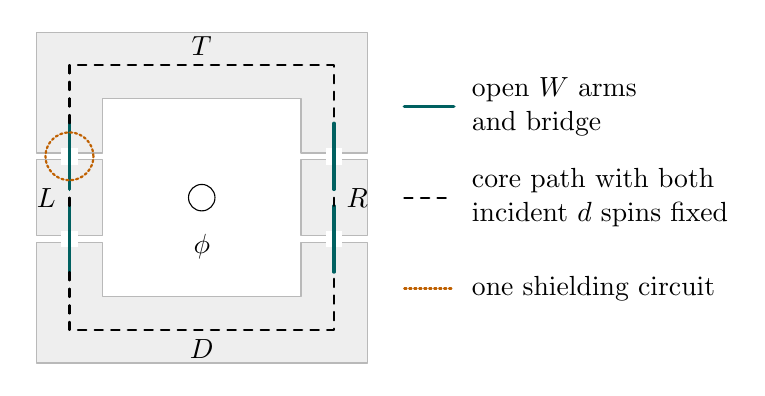
\begin{tikzpicture}[scale=1.05,line cap=round,line join=round]
 \filldraw[fill=gray!13,draw=gray!55]
  (-2,2)--(2,2)--(2,.54)--(1.2,.54)--(1.2,1.2)
  --(-1.2,1.2)--(-1.2,.54)--(-2,.54)--cycle;
 \filldraw[fill=gray!13,draw=gray!55]
  (-2,-2)--(2,-2)--(2,-.54)--(1.2,-.54)--(1.2,-1.2)
  --(-1.2,-1.2)--(-1.2,-.54)--(-2,-.54)--cycle;
 \filldraw[fill=gray!13,draw=gray!55] (-2,-.46) rectangle (-1.2,.46);
 \filldraw[fill=gray!13,draw=gray!55] (1.2,-.46) rectangle (2,.46);
 \foreach \x in {-1.6,1.6}{
  \foreach \y in {-.5,.5}{
   \fill[white] (\x-.1,\y-.1) rectangle (\x+.1,\y+.1);
  }
 }
 \draw[teal!75!black,very thick]
  (-1.6,.1)--(-1.6,.9) (1.6,.1)--(1.6,.9)
  (-1.6,-.1)--(-1.6,-.9) (1.6,-.1)--(1.6,-.9);
 \draw[black,dashed,thick]
  (-1.6,.9)--(-1.6,1.6)--(1.6,1.6)--(1.6,.9)
  (-1.6,-.9)--(-1.6,-1.6)--(1.6,-1.6)--(1.6,-.9)
  (-1.6,-.1)--(-1.6,.1) (1.6,-.1)--(1.6,.1);
 \draw[orange!75!black,densely dotted,thick] (-1.6,.5) circle (.29);
 \node at (0,1.83) {$T$};
 \node at (0,-1.83) {$D$};
 \node at (-1.88,0) {$L$};
 \node at (1.88,0) {$R$};
 \draw (0,0) circle (.16);
 \node[below=5pt] at (0,-.16) {$\supp\phi$};
 \draw[teal!75!black,very thick] (2.45,1.1)--(3.05,1.1);
 \node[right,align=left] at (3.15,1.1) {open $W$ arms\\and bridge};
 \draw[black,dashed,thick] (2.45,0)--(3.05,0);
 \node[right,align=left] at (3.15,0) {core path with both\\incident $d$ spins fixed};
 \draw[orange!75!black,densely dotted,thick] (2.45,-1.1)--(3.05,-1.1);
 \node[right,align=left] at (3.15,-1.1) {one shielding circuit};
\end{tikzpicture}
\caption{The separator after successful trial selection. Gray regions carry
complete $(s,W)$ patterns. Short bridges join the selected open arms across
the gaps; their transverse colors need not be observed. On the dashed core
portions both incident transverse spins are fixed. A surrounding circuit
protects the outside data during each bridge insertion. Only one shielding
circuit and one selected trial per gap are shown.}
\label{fig:screen-separator}
\end{figure}

\begin{lemma}[Selected-arm shielding]
\label{lem:screen-shielding}
For fixed $q$, each trial has conditional two-arm success probability
at least $p(q)>0$, given all earlier trial data. If the first successful
trial is selected, the probability that no trial succeeds is at most
$(1-p(q))^M$. The probability that the selected hole has no surrounding
plus $W$ circuit between scales $Cw$ and $R/10$ is at most $\eta(q)$,
where $\eta(q)\to0$ as $q\downarrow0$. These bounds hold after
averaging over the complete block patterns.
\end{lemma}

\begin{proof}
Reveal previous trials completely before testing the next. Their buffered
neighborhoods are disjoint, so this is exterior $(s,W)$ data for the
current trial. The tube version of \cref{prop:circuits} gives $p(q)$;
the aspect ratios are fixed once $q$ is fixed. A stack of separated
annuli between $Cw$ and $R/10$ gives circuit failure probability at most
$\eta(q)\le Cq^\alpha$ for some $\alpha>0$.

Write $A_j$ for the increasing two-arm event, $G_j$ for the surrounding
plus-circuit event, and $\mathscr H_j$ for the full previous trial
history. Positive association in the remaining law gives
\begin{equation}
 \P(A_j\cap G_j^c\mid\mathscr H_j)
 \le \eta(q)\P(A_j\mid\mathscr H_j).
 \label{eq:screen-relative-shielding}
\end{equation}
If $J$ is the first successful trial, sum this inequality over the
disjoint events $\{J=j\}$. Their total probability is at most one;
there is no factor $M$ in the resulting shielding error. Iterating the
conditional arm bound gives the failure probability. Revealing all
remaining block patterns afterward does not change either averaged
estimate. We do not assert \eqref{eq:screen-relative-shielding} after
conditioning on each individual complete pattern.
\end{proof}

Retain the original marginal law of $S_\delta$. Given this pattern,
select the first successful trial at every gap using a fixed order,
and select its two arms by a deterministic rule. For each selected pair
of arms, choose by a fixed deterministic rule a $W$-lattice path inside
the hole joining their endpoints and meeting the prescribed pattern only
at those plus endpoints. The fixed hole geometry provides such a path for
all sufficiently small meshes. On success, replace the conditional law
by the upper law obtained by pinning these paths open and plus. The new
conditional law is therefore well defined, and its bridge pins are
functions of $S_\delta$.
On unsuccessful patterns leave the conditional law unchanged, couple it
identically to the original law, and take no core-color observations.
Call the resulting law $\mathbb Q_\delta$.

\begin{lemma}[Bridge coupling and exact separation]
\label{lem:screen-bridge-coupling}
The laws $\P_\delta$ and $\mathbb Q_\delta$ can be coupled with their
block patterns identical. Except on probability at most $4\eta(q)$,
their insertion, full exterior data, and all $d$ colors at core sites
outside the shielding disks agree, on the event that all four gaps
have successful trials. Under $\mathbb Q_\delta$, on that success
event one can choose pattern-measurable core paths and condition on
their incident $d$ sites so that the insertion and the full exterior
are conditionally independent given $Y_\delta=(S_\delta,C_\delta)$.
\end{lemma}

\begin{proof}
Fix a block pattern $S$, and write $H(S)$ for success at all four gaps.
On this event let $G_i(S)$ be the plus-circuit event around the selected
hole at gap $i$, and let $\mu_i^S$ be the conditional law after the first
$i$ selected bridges have been pinned, with $\mu_0^S$ the original
conditional law. On unsuccessful patterns put $\mu_i^S=\mu_0^S$ and
$G_i(S)=\Omega$. For two successive laws use the monotone stopping
coupling of \cref{prop:comparison}, searching outward from the newly
pinned hole inside its shielding disk. Stop at the disk's outer boundary
and declare this adjacent coupling unsuccessful if no surrounding plus
circuit has been found. All previously inserted pins are identical in
these two laws.
In the lower law the first plus circuit surrounding that hole is also
open in the upper law. All changed data are inside this common cut. By
\cref{lem:finite-cuts}, the configurations outside it can be sampled
identically, including complementary-component colors. In particular
their exterior color connections are unchanged. The exact neutrality of
the insertion removes any change in the chosen additive height anchor.
If $G_i(S)$ occurs in the lower law, this cut is found inside the
shielding disk, so the required insertion, exterior data, and core colors
outside that disk agree.

To realize these adjacent couplings in the plane, first run each disk-stopped
search in finite flat exhaustions at fixed $\delta$ and $S$, retaining a
binary failure marker. Each conditioning event involves finitely many
prescriptions and has positive plane probability. To verify positivity,
place $S$ and the compatible bridge pins in a larger buffered flat box
with an open plus $W$ perimeter. Keep every prescribed state, put plus
on all remaining $s$ sites, close all remaining interior $W$ edges, and
take all $d$ spins equal. Every factor in \cref{eq:spatial-edge-weight}
is positive because $t\in[1/2,1)$. Let $\mu_{\mathrm{box}}$ denote the
flat law in this box. The restriction $p$ of this filling to a regular
inner core containing the prescriptions is a complete pattern with
$\mu_{\mathrm{box}}(p)>0$. The upper bound
$\mu_{\mathrm{box}}(p)\le C\pi(p)$ in \cref{prop:pattern-comparison}
gives $\pi(p)>0$, and hence positive plane probability for the conditioning
event containing it.

The conditional marginals therefore converge on cylinder events. Extract
a joint limit on the countable product of spin and edge coordinates,
together with the failure marker. Its probability bound passes to the limit,
as does equality of each fixed exterior coordinate on success. Taking their
countable intersection gives equality of the full exterior configuration;
its computable height increments agree as well. Thus this limit has the
plane marginals and the coupling properties just proved in finite volume.

For fixed $S$, the event $G_i(S)$ is now fixed and increasing. The previous
plus pins can only increase its probability. With $\E_S$ denoting
expectation over the original pattern marginal, this gives
\[
 \E_S\!\left[\ind_{H(S)}
       \mu_{i-1}^S\bigl(G_i(S)^c\bigr)\right]
 \le
 \E_S\!\left[\ind_{H(S)}
       \mu_0^S\bigl(G_i(S)^c\bigr)\right]
 \le \eta(q).
\]
The first inequality is the comparison at each fixed pattern; the second
is \cref{lem:screen-shielding} after averaging over the selected trial.
At a fixed mesh the pattern space is finite, so choose these adjacent
conditional couplings measurably in $S$. Apply the displayed estimate to
each of their marginal failure probabilities, then glue the four couplings
and use a union bound. Their searches stay in disjoint buffers, and every
intermediate law retains the original pattern marginal. This proves the
asserted joint coupling.

On a successful pattern, join the outer arm ends through compact cores
of the blocks. The core portions together with the open arms and the
new bridges give a closed walk winding once around $B$ and lying inside
$Q$. Extract a simple winding cycle, with its lattice-width incident
sites, by deterministic loop erasure. On every non-open core edge,
condition on both incident $d$ sites; include the incident sites at the
transitions. Along the arms and bridges no $d$ observation is needed.
Indeed the local factor there is $t\ind_{s_i=s_j}$, independent of
transverse colors. Along a remaining core edge all its $s,W$ data and
the two incident $d$ values are fixed. Every local factor crossing the
cycle is consequently either fixed or independent of the transverse
variables. The Gibbs weight factors into an inside weight and an
outside weight after these observations. This proves conditional
independence. This factorization is made with colors as actual spin
variables, before summing them into cluster-count factors; no hidden
connectivity weight remains across the separator. All observed $d$
sites lie in the compact cores and outside the shielding disks.
\end{proof}

\begin{proof}[Proof of \cref{prop:screened-orthogonality} in the plane]
Truncate the insertion to $[-T,T]$, writing the result as
$X_\delta^{(T)}$, and set
\[
 r(T)=\sup_\delta\E_{\P_\delta}
             |X_\delta-X_\delta^{(T)}|.
\]
The moment bound gives $r(T)\to0$. Suppose the coupling mismatch
probability is $\varepsilon$, and the unsuccessful-pattern probability
is $\zeta$. Duality against bounded functions gives
\begin{align}
 \|\E_{\P_\delta}[X_\delta^{(T)}\mid\mathscr E_\delta]\|_1
 &\le
 \|\E_{\mathbb Q_\delta}
            [X_\delta^{(T)}\mid\mathscr E_\delta]\|_1
       +2T\varepsilon\notag\\
 &\le
 \|\E_{\mathbb Q_\delta}[X_\delta^{(T)}\mid Y_\delta]\|_1
       +2T\varepsilon+2T\zeta\notag\\
 &\le
 \|\E_{\P_\delta}[X_\delta^{(T)}\mid Y_\delta]\|_1
       +4T\varepsilon+2T\zeta.
 \label{eq:screen-bounded-coupling}
\end{align}
For the middle inequality use conditional independence on success and
bound the unsuccessful histories by their probability times $2T$.
The outer inequalities use agreement of the joint insertion and
conditioning data. They do not require equal laws of $Y_\delta$.

By \cref{lem:screen-core-colors}, at each fixed layout the final
conditional norm has limsup at most $r(T)$. The coupling and trial
lemmas give $\varepsilon\le4\eta(q)$ and
$\zeta\le4(1-p(q))^M$. Returning from $X_\delta^{(T)}$ to $X_\delta$
therefore gives
\[
 \limsup_{\delta\downarrow0}
 \|\E[X_\delta\mid\mathscr E_\delta]\|_1
 \le 2r(T)+16T\eta(q)+8T(1-p(q))^M.
\]
Given an error tolerance, first fix $T$ large, then $q$ small, then
$M$ large, and finally fix a layout as in \eqref{eq:screen-scale-order}.
Taking its mesh limit proves \eqref{eq:plane-exterior-orthogonality}.
Only original-law moments have been used; there is no moment assumption
for the artificially pinned law.
\end{proof}

\subsection{Transfer to flat domains}

\begin{proof}[Completion of the proof of
\cref{prop:screened-orthogonality}]
Choose a regular, fixed-width spin ring $A$ between the insertion and
$\partial Q$, with positive clearance from both. Let $R_\delta$ denote
both spins on a lattice-width enlargement of this ring. For a ring
assignment $r$ admitting an interior filling, let $\mathsf K_\delta^r$
be the finite interior spin Gibbs kernel obtained from
\cref{eq:spin-constraint,eq:spin-weight}, with $r$ fixed on the ring and
all factors meeting the interior retained. Define
\[
 g_\delta(r)=\int X_\delta\,\dd\mathsf K_\delta^r,
\]
and put $g_\delta(r)=0$ when no interior filling is admissible.
The neutral insertion is determined by the interior height increments,
so its value in this formula is independent of an additive height anchor.
The finite product weights give this same conditional interior kernel in
every flat domain; the identity also passes from flat exhaustions to the
plane on cylinder events. Thus $g_\delta(R_\delta)$ is a version of the
conditional mean of $X_\delta$ under each of these laws, including on
admissible ring assignments that may have zero plane probability. All
these expectations are finite at each mesh.

Apply the separated-block proof to a slightly smaller surrounding square,
whose exterior contains the ring. All its strict projection clearances
persist under this small change of the surrounding square. Since the ring
data belong to that exterior sigma-field, conditional Jensen gives
$\E_{\P_\delta}|g_\delta(R_\delta)|\to0$, hence convergence in plane
probability. The uniform full-spin
contiguity of \cref{prop:full-contiguity}, on a fixed larger box,
transfers this convergence in probability to the flat laws, even for
mesh-dependent tests of the ring data. The neutral moment estimate in
\cref{lem:screen-pattern-moments}, with no patterns, gives uniform
integrability of these conditional means by conditional Jensen.
Consequently their absolute means tend to zero uniformly over the
flat laws. Finally the Markov property across the ring gives
\[
 \E[X_\delta\mid\mathscr E_\delta(Q)]
    =\E[g_\delta(R_\delta)\mid\mathscr E_\delta(Q)],
\]
and conditional Jensen proves the asserted exterior estimate. Uniformity
can equivalently be checked by taking an arbitrary contradicting
sequence of flat domains; all buffers remain fixed and the same argument
applies. At a random exact cut, the statement is used for the realized
conditional flat law. Subsequent conditioning is not included in this
claim.
\end{proof}

In particular, if finitely many spectator height differences or heights
anchored on an exterior wall are evaluated along paths outside $Q$,
their bounded functions are legitimate exterior observables. Unbounded
products are handled by the moment estimates of the next section. This
is the conditional harmonicity input, with no box shrinking at the
lattice scale.
